% Options for packages loaded elsewhere
\PassOptionsToPackage{unicode}{hyperref}
\PassOptionsToPackage{hyphens}{url}
\PassOptionsToPackage{dvipsnames,svgnames,x11names}{xcolor}
%
\documentclass[
  number,
  preprint]{elsarticle}

\usepackage{amsmath,amssymb}
\usepackage{iftex}
\ifPDFTeX
  \usepackage[T1]{fontenc}
  \usepackage[utf8]{inputenc}
  \usepackage{textcomp} % provide euro and other symbols
\else % if luatex or xetex
  \usepackage{unicode-math}
  \defaultfontfeatures{Scale=MatchLowercase}
  \defaultfontfeatures[\rmfamily]{Ligatures=TeX,Scale=1}
\fi
\usepackage{lmodern}
\ifPDFTeX\else  
    % xetex/luatex font selection
\fi
% Use upquote if available, for straight quotes in verbatim environments
\IfFileExists{upquote.sty}{\usepackage{upquote}}{}
\IfFileExists{microtype.sty}{% use microtype if available
  \usepackage[]{microtype}
  \UseMicrotypeSet[protrusion]{basicmath} % disable protrusion for tt fonts
}{}
\makeatletter
\@ifundefined{KOMAClassName}{% if non-KOMA class
  \IfFileExists{parskip.sty}{%
    \usepackage{parskip}
  }{% else
    \setlength{\parindent}{0pt}
    \setlength{\parskip}{6pt plus 2pt minus 1pt}}
}{% if KOMA class
  \KOMAoptions{parskip=half}}
\makeatother
\usepackage{xcolor}
\setlength{\emergencystretch}{3em} % prevent overfull lines
\setcounter{secnumdepth}{5}
% Make \paragraph and \subparagraph free-standing
\makeatletter
\ifx\paragraph\undefined\else
  \let\oldparagraph\paragraph
  \renewcommand{\paragraph}{
    \@ifstar
      \xxxParagraphStar
      \xxxParagraphNoStar
  }
  \newcommand{\xxxParagraphStar}[1]{\oldparagraph*{#1}\mbox{}}
  \newcommand{\xxxParagraphNoStar}[1]{\oldparagraph{#1}\mbox{}}
\fi
\ifx\subparagraph\undefined\else
  \let\oldsubparagraph\subparagraph
  \renewcommand{\subparagraph}{
    \@ifstar
      \xxxSubParagraphStar
      \xxxSubParagraphNoStar
  }
  \newcommand{\xxxSubParagraphStar}[1]{\oldsubparagraph*{#1}\mbox{}}
  \newcommand{\xxxSubParagraphNoStar}[1]{\oldsubparagraph{#1}\mbox{}}
\fi
\makeatother


\providecommand{\tightlist}{%
  \setlength{\itemsep}{0pt}\setlength{\parskip}{0pt}}\usepackage{longtable,booktabs,array}
\usepackage{calc} % for calculating minipage widths
% Correct order of tables after \paragraph or \subparagraph
\usepackage{etoolbox}
\makeatletter
\patchcmd\longtable{\par}{\if@noskipsec\mbox{}\fi\par}{}{}
\makeatother
% Allow footnotes in longtable head/foot
\IfFileExists{footnotehyper.sty}{\usepackage{footnotehyper}}{\usepackage{footnote}}
\makesavenoteenv{longtable}
\usepackage{graphicx}
\makeatletter
\def\maxwidth{\ifdim\Gin@nat@width>\linewidth\linewidth\else\Gin@nat@width\fi}
\def\maxheight{\ifdim\Gin@nat@height>\textheight\textheight\else\Gin@nat@height\fi}
\makeatother
% Scale images if necessary, so that they will not overflow the page
% margins by default, and it is still possible to overwrite the defaults
% using explicit options in \includegraphics[width, height, ...]{}
\setkeys{Gin}{width=\maxwidth,height=\maxheight,keepaspectratio}
% Set default figure placement to htbp
\makeatletter
\def\fps@figure{htbp}
\makeatother

\usepackage{steinmetz}
\makeatletter
\@ifpackageloaded{caption}{}{\usepackage{caption}}
\AtBeginDocument{%
\ifdefined\contentsname
  \renewcommand*\contentsname{Table of contents}
\else
  \newcommand\contentsname{Table of contents}
\fi
\ifdefined\listfigurename
  \renewcommand*\listfigurename{List of Figures}
\else
  \newcommand\listfigurename{List of Figures}
\fi
\ifdefined\listtablename
  \renewcommand*\listtablename{List of Tables}
\else
  \newcommand\listtablename{List of Tables}
\fi
\ifdefined\figurename
  \renewcommand*\figurename{Figure}
\else
  \newcommand\figurename{Figure}
\fi
\ifdefined\tablename
  \renewcommand*\tablename{Table}
\else
  \newcommand\tablename{Table}
\fi
}
\@ifpackageloaded{float}{}{\usepackage{float}}
\floatstyle{ruled}
\@ifundefined{c@chapter}{\newfloat{codelisting}{h}{lop}}{\newfloat{codelisting}{h}{lop}[chapter]}
\floatname{codelisting}{Listing}
\newcommand*\listoflistings{\listof{codelisting}{List of Listings}}
\makeatother
\makeatletter
\makeatother
\makeatletter
\@ifpackageloaded{caption}{}{\usepackage{caption}}
\@ifpackageloaded{subcaption}{}{\usepackage{subcaption}}
\makeatother
\journal{Journal Name}

\ifLuaTeX
  \usepackage{selnolig}  % disable illegal ligatures
\fi
\usepackage[]{natbib}
\bibliographystyle{elsarticle-num}
\usepackage{bookmark}

\IfFileExists{xurl.sty}{\usepackage{xurl}}{} % add URL line breaks if available
\urlstyle{same} % disable monospaced font for URLs
\hypersetup{
  pdftitle={Prática de Adaptação de Impedância},
  pdfauthor={Bruno Alexandre Fraga},
  pdfkeywords={Robustez, Adaptação de impedância, Análise estatística},
  colorlinks=true,
  linkcolor={blue},
  filecolor={Maroon},
  citecolor={Blue},
  urlcolor={Blue},
  pdfcreator={LaTeX via pandoc}}


\setlength{\parindent}{6pt}
\begin{document}

\begin{frontmatter}
\title{Prática de Adaptação de Impedância \\\large{Laboratório 06} }
\author[1]{Bruno Alexandre Fraga%
%
}
 \ead{bruno.fraga@posgrad.ufsc.br} 

\affiliation[1]{organization={Universidade Federal de Santa
Catarina, Departamento de Engenharia Elétrica e
Eletrônica},addressline={R. Delfino
Conti},city={Florianópolis},postcode={88040-370},postcodesep={}}

\cortext[cor1]{Corresponding author}

        
\begin{abstract}
Este trabalho tem por objetivo consolidar a técnica de projeto de redes
de casamento de impedância, em especial a técnica pela rede L. Para
isso, é proposto realizar o casamento de impedância da saída de um
amplificador para uma carga de 50 \(\Omega\) de modo que a eficiência da
potência dissipada na carga seja de 80\%. Após algumas análises o
projeto foi concluído com sucesso e realizada uma simulação Monte Carlo
com 100 iterações para verificar a robustez do projeto por técnicas
estatísticas. Os resultados obtidos foram brevemente discutidos.
\end{abstract}





\begin{keyword}
    Robustez \sep Adaptação de impedância \sep 
    Análise estatística
\end{keyword}
\end{frontmatter}
    

\section{Prelab}\label{prelab}

\subsection{Potência dissipada na
carga}\label{potuxeancia-dissipada-na-carga}

A potência dissipada na carga, \(P_L\), é dada pela seguinte expressão

\[
  P_L=\frac{V_L\cdot I_L^*}{2}
\]

em que \(V_L\) é a tensão na carga e \(I_L^*\) o conjugado da corrente
que passa pela mesma.

Como o circuito está todo em paralelo, a tensão na carga é a mesma
tensão do circuito todo, ou seja, \(V_L=V_s\), como pode-se verificar na
Fig.~\ref{fig-original-circuit}.

\begin{figure}

\centering{

\includegraphics{../images/circuit-original.png}

}

\caption{\label{fig-original-circuit}Circuito para medição da admitância
total}

\end{figure}%

Com base nisso, percebe-se que

\[
  P_L=\frac{V_s\cdot V_s^*}{2R_L}
\]

pois \(I_L=V_s/R_L\). E assim obtém-se que

\[
  V_s=\frac{I_s}{Y_N}
\]

em que \(Y_N\) é a admitância de Norton do circuito. Essa admitância é
calculada como se segue

\[
  \begin{split}
    Y_N&=R_s^{-1}-jX_s^{-1}+Y_L\implies\\
    &=\frac{X_s\left(1+Y_LR_s\right)-jR_s}{X_sR_s}
  \end{split}
\]

dessa forma, obtém-se que a tensão em cima da carga é de

\[
  V_s=\frac{I_sX_sR_s}{X_s\left(1+Y_LR_s\right)-jR_s}
\]

Substituindo \(X_s=\omega L_s\), obtém-se

\[
  V_s=\frac{I_s\omega L_sR_s}{\omega L_s\left(1+Y_LR_s\right)-jR_s}
\]

Assim, a forma mais simples de se calcular a potência sobre a carga é
obter o valor de \(V_s\), e calcular a potência por meio da expressão já
obtida anteriormente.

\subsection{Eficiência}\label{eficiuxeancia}

Tendo o valor de \(V_s\) já definido, a obtenção do valor da potência da
fonte do circuito, \(P_s\) é simples, como pode-se verificar a seguir

\[
  P_s=\frac{V_sI_s^*}{2}
\]

A expressão de \(V_s\) já foi estabelecida e \(I_s\) é uma hipótese do
problema.

A fim de se verificar as expressões obtidas, é realizada simulação de
parâmetros S para obter a impedância do circuito. Essa comparação é
apresentada na Tab~\ref{tbl-admitances}.

\begin{longtable}[]{@{}ll@{}}
\caption{Admitâncias simulada e
calculada}\label{tbl-admitances}\tabularnewline
\toprule\noalign{}
\(Y_N\) simulado (mS) & \(Y_N\) calculado (mS) \\
\midrule\noalign{}
\endfirsthead
\toprule\noalign{}
\(Y_N\) simulado (mS) & \(Y_N\) calculado (mS) \\
\midrule\noalign{}
\endhead
\bottomrule\noalign{}
\endlastfoot
\(28,8\phase{-13.3^{\circ}}\) & \(28,8\phase{-13.3^{\circ}}\) \\
\end{longtable}

A impedância referente a essa admitância (\(Y_N^{-1}\)) que foi simulada
pode ser verificada na Fig~\ref{fig-admita-smith}.

\begin{figure}

\centering{

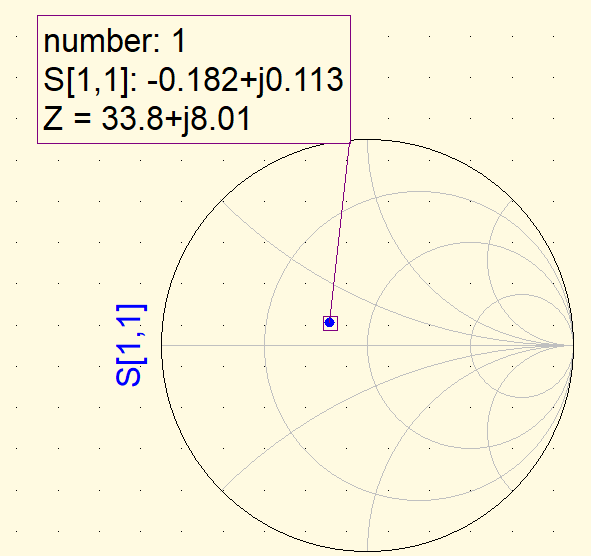
\includegraphics{../images/admita-smith.png}

}

\caption{\label{fig-admita-smith}Circuito para medição da admitância
total}

\end{figure}%

Com base em tudo que foi discutido até então, pode-se realizar a análise
da eficiência \(\eta=P_s/P_L\) pela resistência da carga, \(R_L\). A
curva obtida pode ser visualizada na Fig~\ref{fig-admita-smith}.

\begin{figure}

\centering{

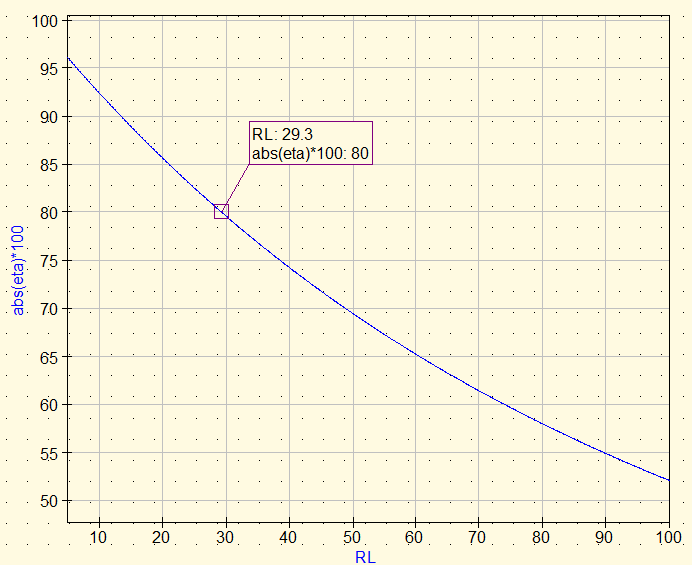
\includegraphics{../images/load-80eff.png}

}

\caption{\label{fig-load-80eff}Circuito para medição da admitância
total}

\end{figure}%

Além da curva, também foi evidenciado o ponto em que a eficiência de
80\% é atingido, ou seja \(29,3\;\Omega\).

\section{Rede de adaptação}\label{rede-de-adaptauxe7uxe3o}

Para que o circuito fornecido pelo problema realize uma dissipação de
80\% da potência fornecida pela fonte, essa carga deve ser de 29,3
\(\Omega\). Entretanto, a carga do problema é de 50 \(\Omega\), sendo
assim, o circuito equivalente do amplificador deve enxergar uma
resistência de carga de 29,3 \(\Omega\) ao invés de 50 \(\Omega\). Essa
adaptação é realizada por meio da rede tipo L
\citep{steer2019microwavev3}.

Para essa tarefa, imaginou-se que a impedância de \(R_s=50\;\Omega\)
deva ser adaptada para \(R_L=29,3\;\Omega\). Assim, obtém-se

\[
  Q=\sqrt{\frac{R_s}{R_L}-1}=0,84
\]

Como o circuito é o modelo equivalente de um amplificador, optou-se por
bloquear a passagem de AC e, assim, utilizar a topologia do capacitor em
paralelo. A impedância reativa desse capacitor é de

\[
\begin{split}
  X_c&=QR_L=24,6\;\Omega\implies\\
  C&=2,7\;\text{pF}
\end{split}
\]

e a impedância reativa do indutor em paralelo é dada por

\[
\begin{split}
  X_L&=\frac{R_s}{Q}=59,5\;\Omega\implies\\
  L&=3,9\;nH
\end{split}
\]

O circuito da rede de adaptação em questão pode ser visualizado na
Fig.~\ref{fig-L-net}.

\begin{figure}

\centering{

\includegraphics{../images/L-net.png}

}

\caption{\label{fig-L-net}Circuito para medição da admitância total}

\end{figure}%

Esse circuito possui uma impedância de 29,3 \(\Omega\), conforme pode
ser visualizado na Fig.~\ref{fig-impedance-smith-Lnet}.

\begin{figure}

\centering{

\includegraphics{../images/impedance-smith-Lnet.png}

}

\caption{\label{fig-impedance-smith-Lnet}Circuito para medição da
admitância total}

\end{figure}%

As Fig.~\ref{fig-admit-allfreqe} e Fig.~\ref{fig-reflex-allfreq}
apresentam a admitância e o coeficiente de reflexão da rede de adaptação
ao longo de um amplo espectro de frequência (100 MHz a 10 GHz), com a
carga de 50 \(\Omega\).

\begin{figure}

\centering{

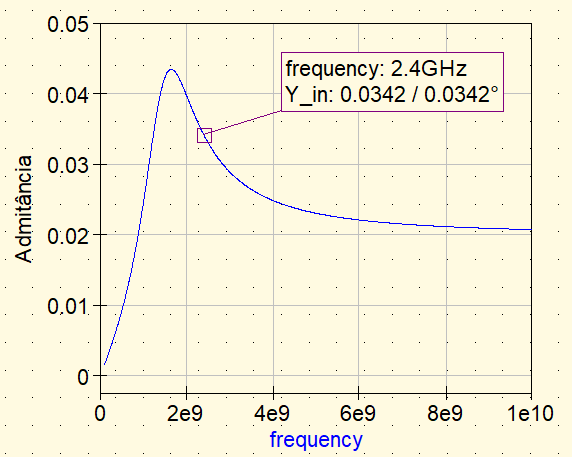
\includegraphics{../images/admit-allfreqe.png}

}

\caption{\label{fig-admit-allfreqe}Circuito para medição da admitância
total}

\end{figure}%

\begin{figure}

\centering{

\includegraphics{../images/reflex-allfreq.png}

}

\caption{\label{fig-reflex-allfreq}Circuito para medição da admitância
total}

\end{figure}%

\section{Teste da rede L ao circuito equivalente do
amplificador}\label{teste-da-rede-l-ao-circuito-equivalente-do-amplificador}

Ao finalizar os testes e medições da rede L isoladamente, essa rede é
acoplada ao circuito equivalente do amplificador. E pode-se perceber,
pela Fig.~\ref{fig-test-Lnet}, que a rede projetada adequou corretamente
a impedância do amplificador, de modo que a eficiência da potência
dissipada na carga foi de 80\%.

\begin{figure}

\centering{

\includegraphics{../images/test-Lnet.png}

}

\caption{\label{fig-test-Lnet}Circuito para medição da admitância total}

\end{figure}%

\section{Simulação Monte Carlo}\label{simulauxe7uxe3o-monte-carlo}

Para garantir a robustez do projeto, analiza-se a simulação Monte Carlo
e pode-se verificar estatisticamente se o projeto atende a alguns
padrões estabelecidos (como o de ter os resultados dentro de uma faixa
de 3 vezes o desvio padrão da distribuição).

A Fig.~\ref{fig-monte-carlo} mostra o arranjo utilizado para realizar a
simulação Monte Carlo. Os dados obtidos por meio dessa simulação foram
exportados e serão apresentados a seguir.

\begin{figure}

\centering{

\includegraphics{../images/monte-carlo.png}

}

\caption{\label{fig-monte-carlo}Circuito para medição da admitância
total}

\end{figure}%

Pela Fig.~\ref{fig-efficiency-points} pode-se verificar que a média da
eficiência do circuito, com componentes de 5\% de tolerância foi de
79\%, sendo que, exatamente todas as amostras, no espaço amostral de 100
testes, ficaram dentro dos 3\(\sigma\), o que é um excelente resultado,
tendo em vista que, com base nesse teste, pode-se concluir inicialmente
que 99,7\% dos casos o circuito terá uma variação máxima de 3\(\sigma\)
a mais e a menos em relação à média de 79\%. Isso significa que os
valores podem variar, no máximo, de 75,83\% a 82,15\%.

\begin{figure}

\centering{

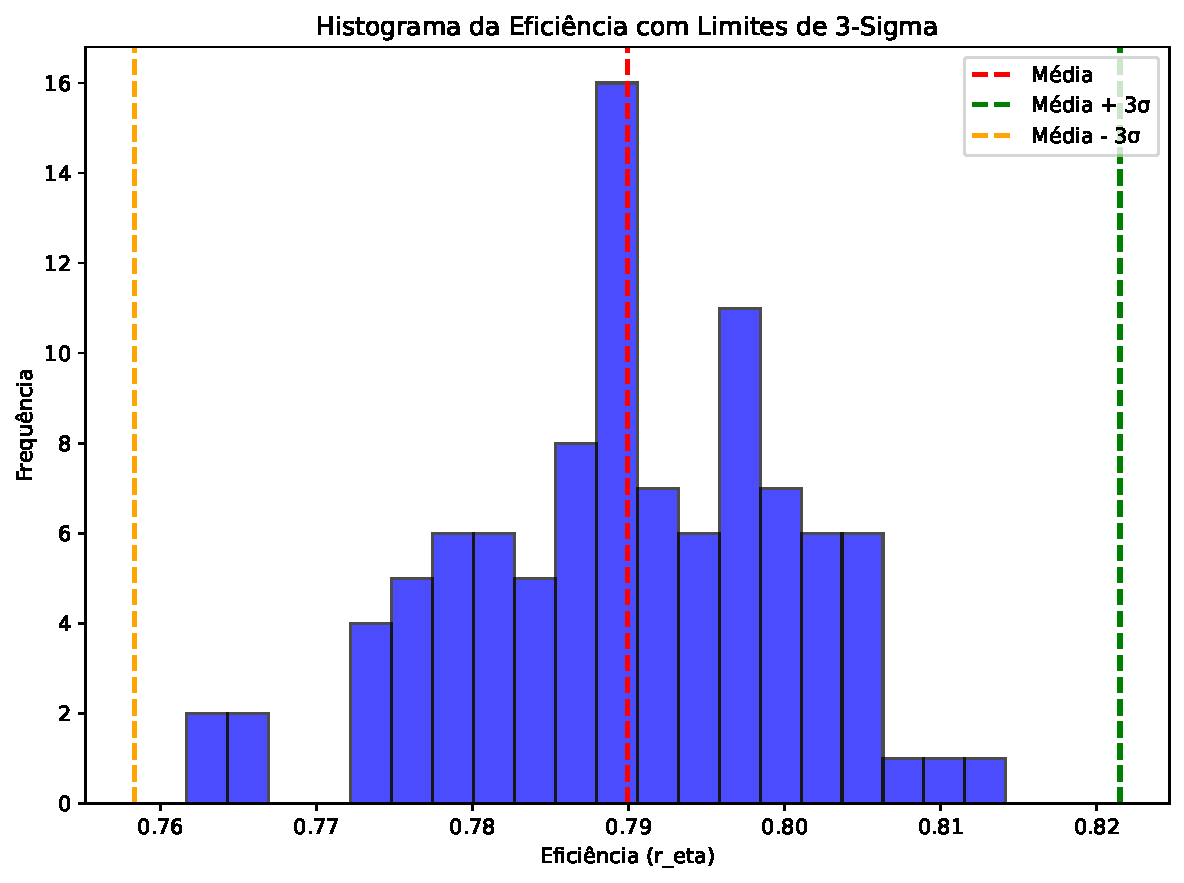
\includegraphics{article_files/figure-pdf/fig-efficiency-points-output-1.pdf}

}

\caption{\label{fig-efficiency-points}A meaningless scatterplot}

\end{figure}%

A potência dissipada na carga, por sua vez, apresenteou um comportamento
em que a média da potência é de 93,7 mW, sendo que os 99,7\% das
amostras (3\(\sigma\)) ficaram dentro de um intervalo de 86,4 mW e 100
mW.

\begin{figure}

\centering{

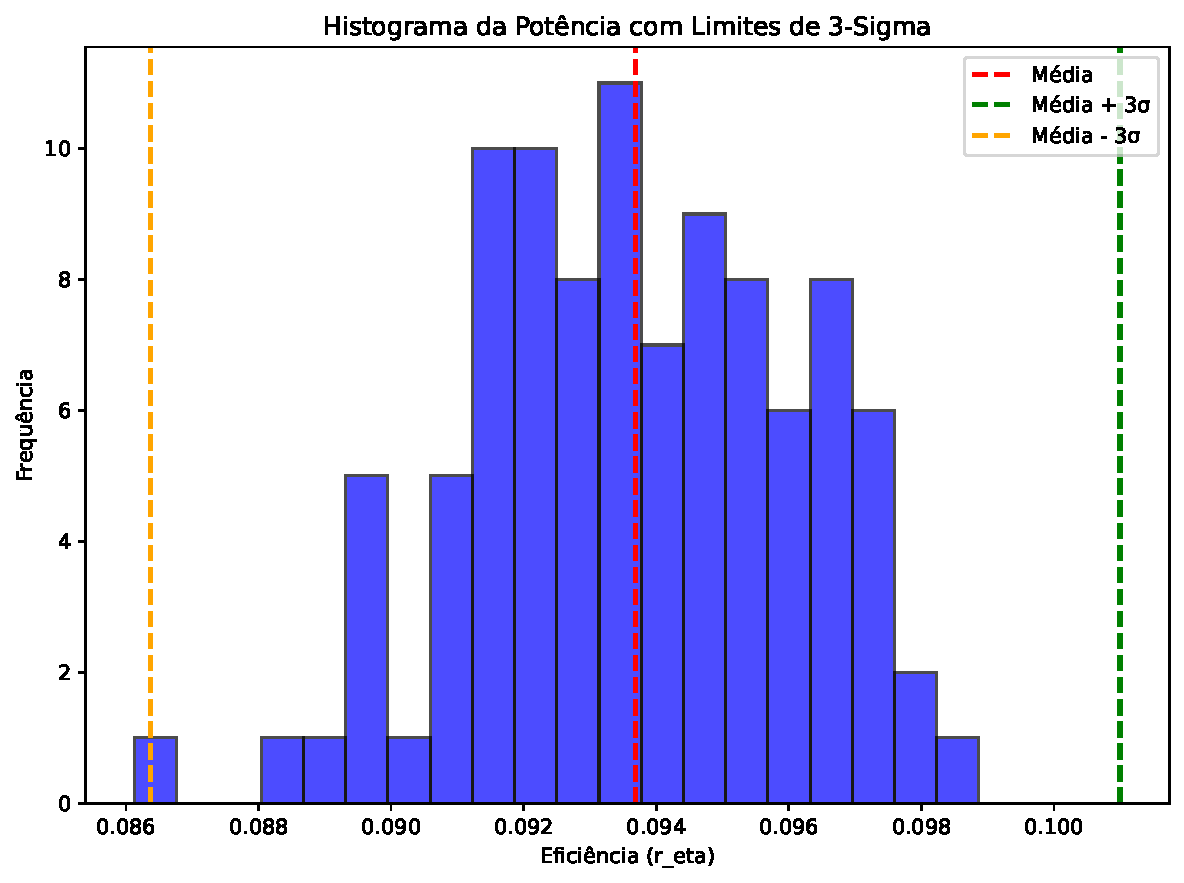
\includegraphics{article_files/figure-pdf/fig-power-points-output-1.pdf}

}

\caption{\label{fig-power-points}A meaningless scatterplot}

\end{figure}%

\section{Discussão}\label{discussuxe3o}

Com essa atividade, tive a oportunidade de consolidar o conhecimento de
adaptação de impedâncias pela técnica da rede L. Entretanto, a parte de
mais valor da atividade é a análise estatística que deve ser analisada
para verificar a robustez do projeto. Eu já havia ouvido falar da
simulação Monte Carlo e até já havia performado algumas análises no
software Keysight ADS, como parte de um tutorial, mas não tinha muita
noção do motivo e da importância da simulação. Além disso, eu
particularmente tenho negligenciado a estatística e, com base no que foi
verificado nesta atividade, isso não é correto, uma vez que nada no
mundo real é ideal e, em se tratando de circuitos de radiofrequência,
pequenas não-idealidades podem causar comportamentos muito
significativos.

Outro ponto um pouco menos importante é que esse relatório foi feito
utilizando a tecnologia Quarto, apresentada em sala de aula como uma
ferramenta essencial para gerar relatórios e documentação acadêmica.

Um dos pontos que ficaram um pouco mal documentados é em relação à
análise estatística dos resultados obtidos. Como comentei, minha parte
de estatística foi um pouco negligenciada, logo tenho uma certa
necessidade de relembrar e aprofundar os conceitos. Minha sugestão de
como eu posso mitigar essa lacuna no meu conhecimento é analisar com
muito mais atenção quando alguns valores e conceitos estatísticos forem
apresentados em algum artigo ou bibliografia (eu costumo passar bem por
cima nessas seções), bem como em manter como padrão, realizar análises
de robustez nos projetos que tenho a oportunidade de trabalhar.


\renewcommand\refname{References}
  \bibliography{bibliography.bib}



\end{document}
